\chapter{Backend}

En esta sección voy a hablar de \textbf{la implementación del microservicio de geolocalización}, el backend del sistema de auxilio.
\section{Lenguaje de programación}
He decidido usar \textbf{Typescript.} Es un lenguaje de tipado gradual que transpila a Javascript.
Como ventajas sobre Javascript:
\begin{itemize}
	\item Mejor \textit{developer experience}, sobre todo gracias al autocompletado.
	\item \textbf{Detección de errores precoz gracias a los tipos.}
\end{itemize}
Es cierto, sin embargo, que añade más complejidad en el setup de desarrollo (y también en el de despliegue) del que hablo en la sección \ref{sec:dev}. \\ \\
\textbf{Considero que es un \textit{sweet spot} entre la excesiva libertad en Javascript y la rigidez de lenguajes tipados estrictos como Java o C\#.} \\ \\

\textbf{Como runtime he elegido Node.} Utiliza una sola hebra con E/S no bloqeuante, lo cual se ajusta bien al tipo 
de peticiones que se atienden en este backend (sin cómputos extensos).  \\ \\
Como alternativa, podría haber elegido Deno, pero no tiene un ecosistema aún tan desarrollado.

\section{Framework}
\textbf{La API será, por simplicidad, REST.} Necesitamos un framework para implementar esta interfaz. \\

\textbf{He decido usar Express. Es un framework \textit{unopinionated} muy consolidado.} Esto tiene importancia en la 
arquitectura limpia que explico en la sección \ref{sec:clean}. \\
Otras alternativas que he considerado son: Koa, Fastify o Hapi.

\section{Setup de desarrollo}\label{sec:dev}

He invertido tiempo para tener \textbf{un entorno de desarrollo replicable por cualquiera que esté interesado en trabajar en este proyecto.}
Por eso, he usado Docker y Docker Compose. He creado un \textit{Dockerfile} que encapsula el microservicio. 
\\ Por último, en Docker Compose arranco y comunico el microservicio y los otros procesos (base de datos y pub/sub). \\ \\
\textbf{Las instrucciones para iniciar un entorno de desarrollo son las siguientes:}

\begin{enumerate}
	\item En el archivo \textit{.env.template} están recogidas las variables de entorno que hacen falta para configurar este microservicio.
Podemos simplemente copiar este archivo a otro de nombre \textit{.env} y \textit{dotenv} se encargará de usarlas (ver sección \ref{sec:config}).
\item También necesitamos un archivo \textit{serviceAccountKey.json} que se puede obtener en Firebase Cloud Messaging y que hay que situar en este directorio. 
(En el .gitignore está declarado este archivo porque contiene claves privadas.)
\item Una vez hecho esto, simplemente ejecutamos: \textbf{\textit{docker-compose up}}.
\end{enumerate}

\section{Base de datos}

Necesito una base de datos que \textbf{soporte un gran volumen de operaciones y permita consultas basadas en localizaciones geográficas.} \\ \\
\textbf{En el CAP Theorem necesito la A (de availability) y la P (de partition tolerance), sacrificando la consistencia.}
\\
En esta base de datos se almacenará de manera periódica la ubicación de cada uno de los usuarios con el fin de una consulta posterior, que nos permita saber qué usuarios
están cerca de una persona que necesita ayuda. Por ello, es más que suficiente la consistencia eventual.

\subsection{Opciones}

\begin{itemize}
	\item \textbf{MongoDB tiene buen soporte para \textit{geo-queries}}, de hecho vienen ya instaladas, sin embargo, \textbf{prioriza la consistencia antes que la disponibilidad.}
\item \textbf{PostgreSQL}, con PostGIS, \textbf{también soporta bien este tipo de consultas, pero prioriza la consistencia a la tolerancia a la partición.} 
\item \textbf{CouchDB, Dynamo y Cassandra son sistemas con alta disponibilidad y tolerancia a la partición.} CouchDB es la mejor opción porque Dynamo es privativa y Cassandra es más adecuada para aplicaciones con más
escrituras que actualizaciones. 
\end{itemize}



Tras usar CouchDB me di cuenta de que \textbf{el soporte para queries de geolocalización} \href{https://docs.couchdb.org/en/stable/ddocs/search.html?highlight=geospatial#geographical-searches}{no es bueno}.

\textbf{Acabe optando por MongoDB} que \href{https://stackoverflow.com/questions/25734092/query-locations-within-a-radius-in-mongodb}{sí tiene buen soporte}.

Además, puedo habilitar la escritura en replicas para cambiar la consistencia estricta por consistencia eventual y tener más disponibilidad. \href{https://stackoverflow.com/questions/11292215/where-does-mongodb-stand-in-the-cap-theorem}{Explicado aquí.}

\subsection{Configuración de MongoDB}

En el archivo \textit{mongo-init.js} creo el usuario que se va a utilizar desde el microservicio y el índice "2dsphere". 
En Docker Compose lo monto como volumen para que lo pueda usar la instancia que se declara ahí.

\section{Arquitectura limpia}\label{sec:clean}

He tratado de mantener en todo momento \textbf{el dominio desacoplado de los detalles de infraestructura, de la interfaz de usuario y de cualquier framework.}
\begin{figure}[H]
	\centering	
	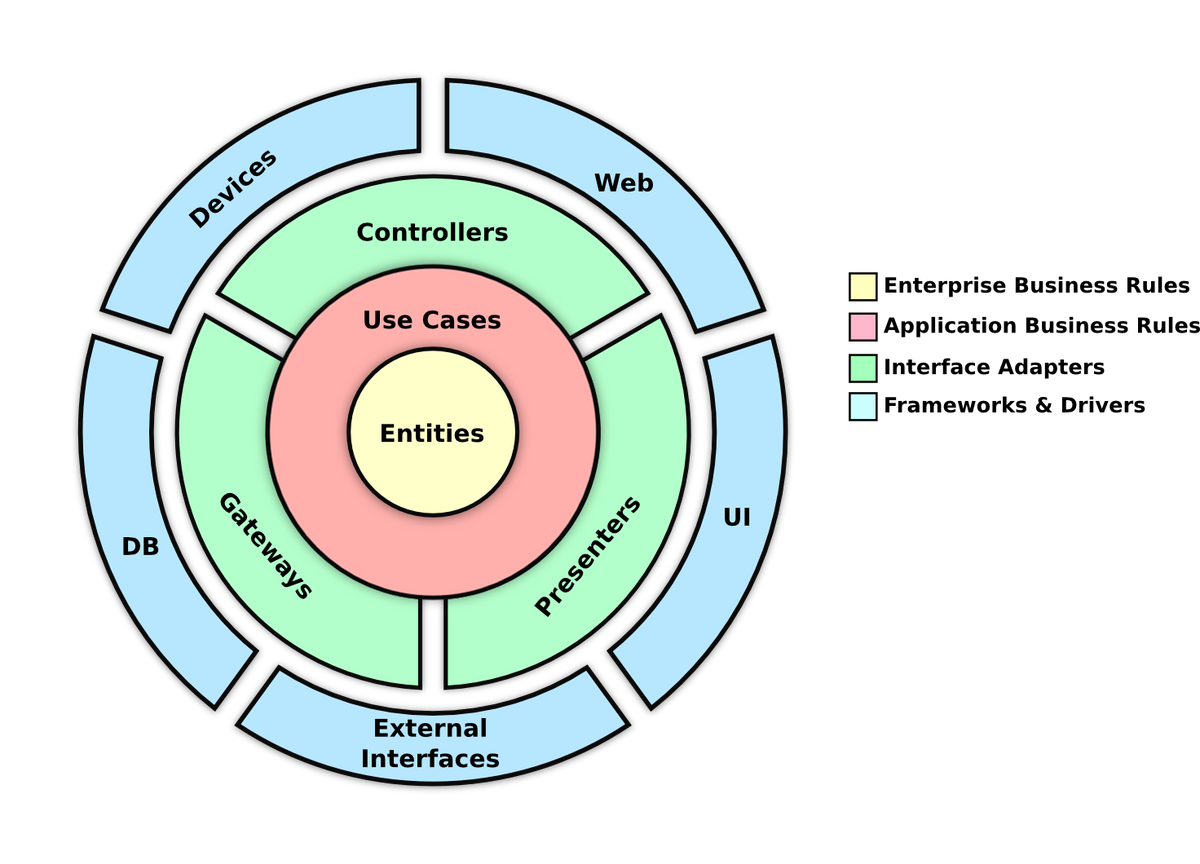
\includegraphics[scale=0.3]{clean_arc.png}
	\end{figure}

Tenemos tres capas bien diferenciadas:
\subsection{Aplicación}
En este caso es una \textbf{API REST implementada con Express.} Toma peticiones HTTP, extrae la información, la valida, usa métodos expuestos del dominio y devuelve información.
Aparte, también hay un endpoint websocket que explico en la subsección \ref{subsec:websocket}. \\
Considero importante separar bien esta capa del servicio que consume. Con esto, sería sencillo dejar de usar 
REST para utilizar \textit{SOAP} o \textit{GraphQL}, por ejemplo.

\subsection{Dominio}
\textbf{Tipos y casos de uso que pertenecen exclusivamente al dominio.}
Cuando estos casos de uso necesitan utilizar un servicio de infraestructura como el de persistencia, por ejemplo,
\textbf{se depende exclusivamente de una interfaz que describe esa función y se inyecta en tiempo de ejecución un servicio que la implemente (inyección de dependencias).}
\begin{figure}[H]
	\centering	
	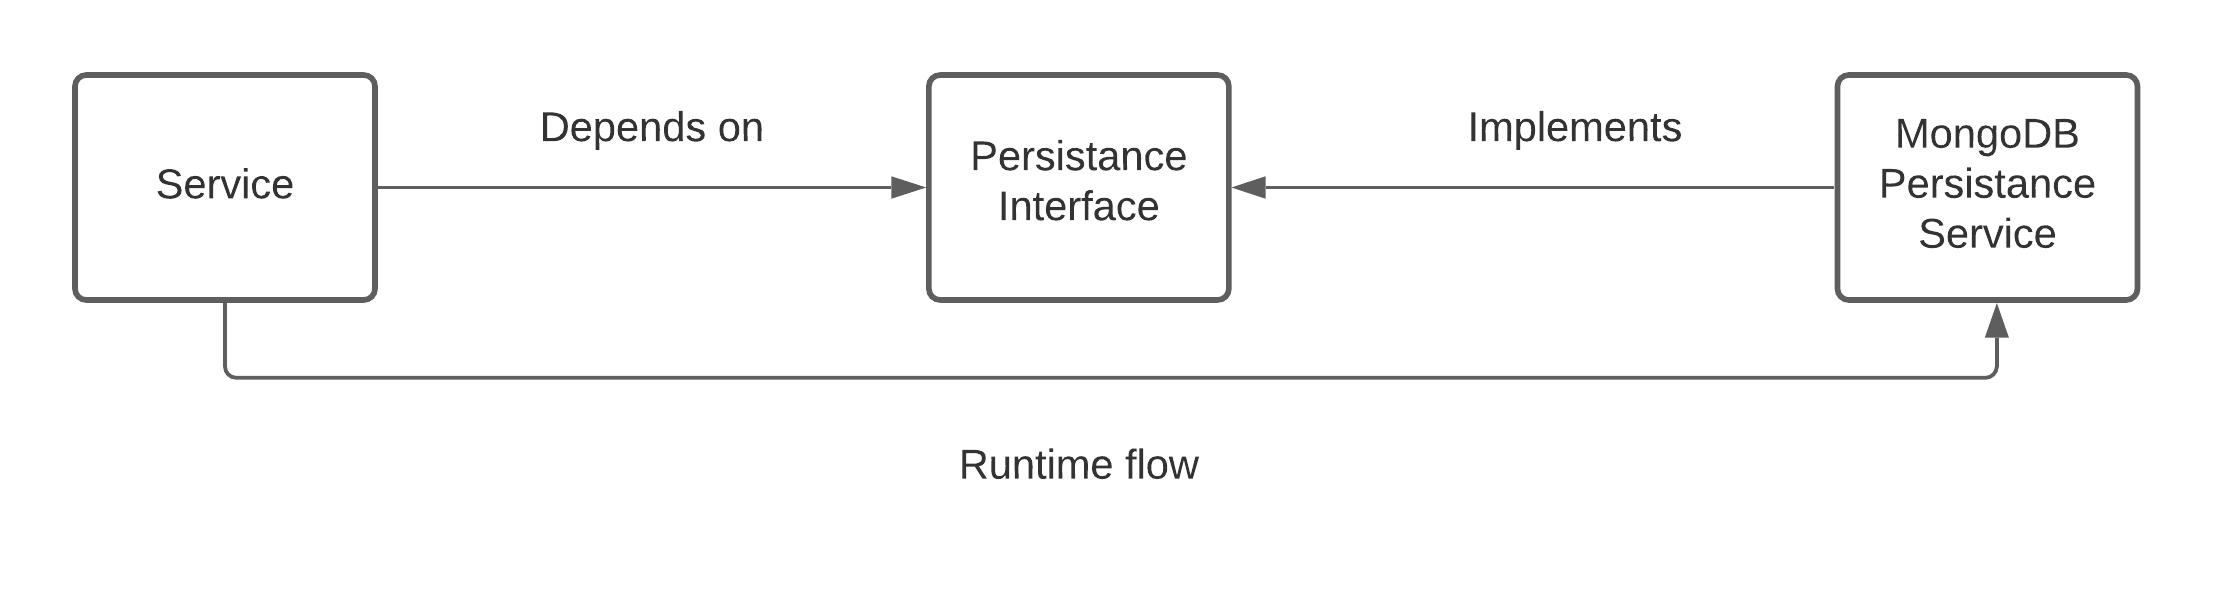
\includegraphics[scale=0.7]{di.png}
	\caption{Inyección de dependencias}
	\end{figure}

Asimismo, \textbf{esta separación incrementa mucho la testeabilidad del microservicio,} porque las únicas dependencias
que puede tener esta capa forman parte del lenguaje de programación. Podemos usar \textit{mocks} para implementar
las interfaces de infraestructura y probar todas las posibles respuestas de estos servicios. \\ \\
Por último, he comentado concienzuadamente las interfaces con \textbf{js-doc} para facilitar la implementación de otros servicios.
\begin{figure}[H]
	\centering	
	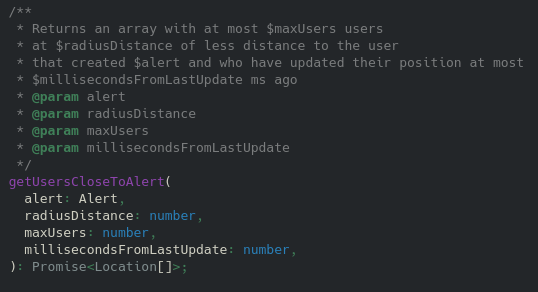
\includegraphics[scale=0.9]{jsdoc.png}
	\end{figure}

\subsection{Infraestructura} 
Son servicios que implementan las interfaces de las que acabo de hablar.
En este capa está la lógica para comunicarse con los distintos servicios: Bases de datos, mensajería, etc...
\begin{figure}[H]
	\centering	
	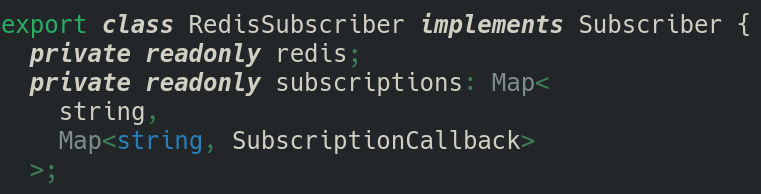
\includegraphics[scale=0.6]{imp.png}
	\end{figure}


\section{Operaciones}

Descripción en líneas generales de los tipos de peticiones que debe atender el backend:

\subsection{Crear/Actualizar ubicación}\label{op:ubi}
Toma unas coordenadas y un id de usuario y persiste en la base de datos.
Esta operación es indispensble para avisar a los usuarios cercanos a una emergencia y para 
actualizarles sobre la posición de una víctima (publicando la ubicación actualizada en el pub/sub, sección \ref{sec:pubsub}).

\subsection{Crear alerta}
Verificando antes que el usuario no tiene ya otra alerta en curso, la persiste.
Busca todos los usuarios cercanos que hayan actualizado su ubicación recientemente y les avisa. Para hacer
esta consulta rápidamente, la operación \ref{op:ubi} indexa las ubicaciones.
Mientras siga en estado activo, se verifica que el usuario sigue actualizando su ubicación, de lo contrario la alerta pasa a estado inactivo.

\subsection{Escuchar alerta}\label{subsec:websocket}
Los usuarios a los que se ha avisado de la alerta pueden empezar a escuchar actualizaciones de la alerta,
ya sea porque el usuario que la creó cambia su posición o porque la alerta es ya inactiva. \\
Para esto:
\begin{enumerate}
	\item El cliente y el servidor mantienen un websocket abierto.
	\item Se subscribe a los cambios en la alerta o en la ubicación.
	\item Cuando estos cambios se producen, se emiten por el websocket al cliente.
	\item Si la alerta pasa a estado inactivo, el websocket se cierra y se desubscribe.
\end{enumerate}
\textbf{Utilizo websockets porque permite al servidor hacer "push" de información sin que el cliente tenga que hacer "polling".}
He considerado que podría utilizar otros protocolos como SSE (server sent events) y una implementación más peer to peer con WebRTC por ejemplo, conectando directamente los dispositivos interesados.

Es cierto que quitaría carga al servidor, pero también aumentaria la complejidad.

\subsection{Borrar alerta}
Se marca una alerta existente como inactiva. Si hay usuarios pendientes de esta alerta, se les avisa.


\section{Pub/Sub}\label{sec:pubsub}
\textbf{Al añadir websockets}, teniendo en cuenta que queremos tener escalado horizontal en este servicio,
\textbf{necesitamos un sistema de publicación/subscripción.} \\
Para ello, \textbf{he elegido Redis}, que cuenta con una interfaz muy simple. Como librería, ioredis, 
que es muy robusta y rápida.\\ \\

Para escalar, tendríamos que añadir más instancias del microservicio y potenciar el cluster de redis para la comunicación entre ellas.

\begin{figure}[H]
	\centering	
	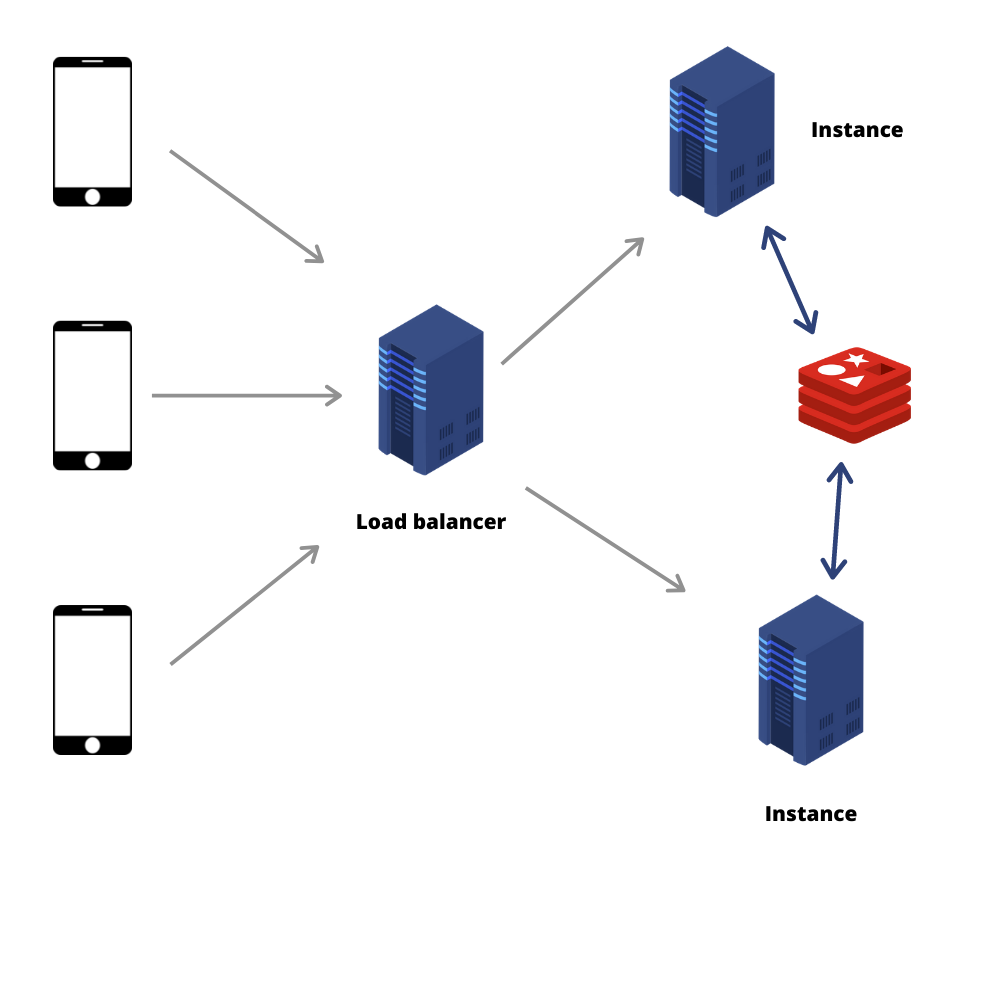
\includegraphics[scale=0.4]{pubsub.png}
	\end{figure}

\textbf{Por cada instancia del microservicio, tenemos dos conexiones a Redis:}
\subsection{Publisher}

Este servicio simplemente se conecta a Redis y \textbf{publica entidades en el momento en el que se modifican} (ubicaciones y alertas).
Publica al canal definido con el id de la entidad, esta misma serializada.

\subsection{Subscriber}
Este servicio es algo más sofisticado. \textbf{Mantiene en un Map los canales a los que está subscrito y 
para cada canal todas las subscripciones.} Estas mismas tienen un id para manejar la desubscripción (generado en tiempo de creación) y 
el callback que hay que ejecutar cuando llega una publicación para esa subscripción. 
\begin{figure}[H]
	\centering	
	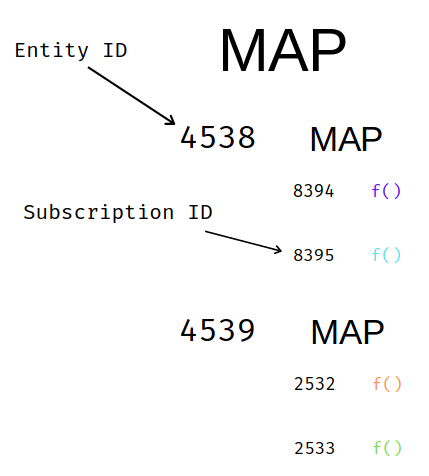
\includegraphics[scale=0.8]{map.png}
	\caption{Estructura de datos en Subscriber}
	\end{figure}
Cuando un websocket se cierra, las subscripciones asociadas desaparecen de esta estructura.
\section{Envío de notificaciones}\label{sec:fibpre}
\textbf{Para avisar a las personas cercanas de que alguien necesita ayuda, tenemos que tener la habilidad de enviar
notificaciones push.} Para esto he usado Firebase Cloud Messaging, del que hablo más en la sección \ref{sec:fib}.

\section{Tests}\label{sec:tests}
En este microservicio uso Jest y Supertest para \textbf{testear las capas de aplicación y dominio, con mocks de la capa de infraestructura.} \\ \\
Como próximos pasos, deberíamos implementar tests unitarios para la capa de dominio y especialmente la de infraestructura.
\begin{figure}[H]
	\centering	
	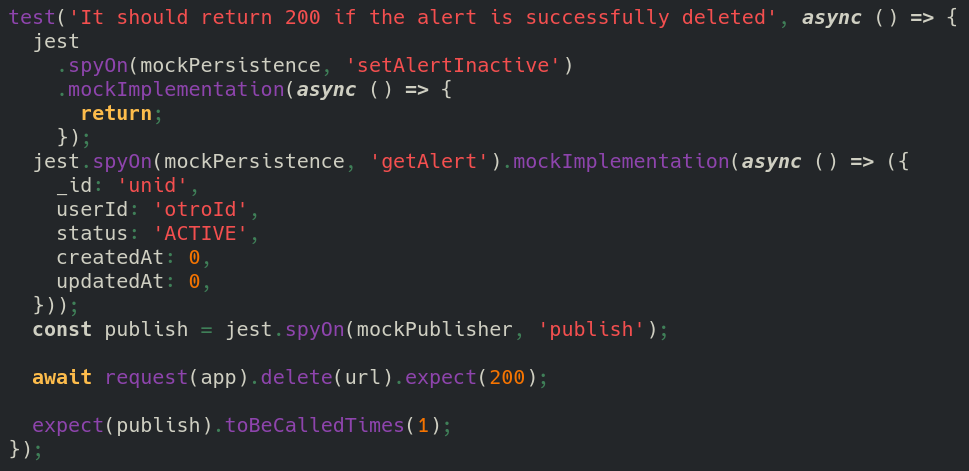
\includegraphics[scale=0.5]{test.png}
	\end{figure}

\section{Configuración}\label{sec:config}
\textbf{Las variables de configuración se definen mediante variables de entorno.} Para desarrollo uso \textit{dotenv}, 
que las carga de un archivo de configuración.
\begin{figure}[H]
	\centering	
	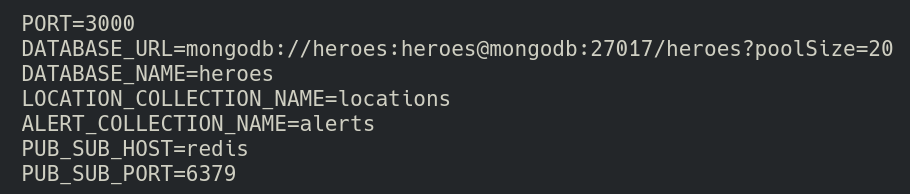
\includegraphics[scale=0.5]{env.png}
	\end{figure}

	Por otro lado, \textbf{los parámetros de configuración que tengan que ver con la lógica
	de negocio, los he declarado y documentado en el servicio de dominio.}

\begin{figure}[H]
	\centering	
	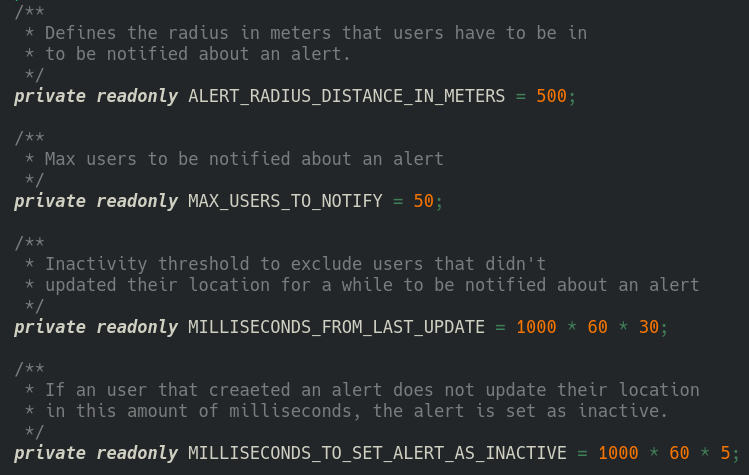
\includegraphics[scale=0.6]{conf.png}
	\end{figure}



\section{Otras herramientas}\label{sec:tools}
Otras herramientas que he utilizado en esta parte son:
\begin{itemize}
	\item \textbf{Express-validator} para validar los cuerpos de las peticiones HTTP
	\item \textbf{ESLint} para mantener las buenas prácticas.
	\item \textbf{Prettier} para el formateo del código.
	\item \textbf{Nodemon} para reiniciar el microservicio cada vez que hay cambios durante el desarrollo.
	\item \textbf{Concurrently} para ejecutar con un solo comando (\textit{npm run dev}) el watcher de Typescript y Nodemon.
\end{itemize}